\documentclass{article}
\usepackage[utf8]{inputenc}
\usepackage{amsmath}
\usepackage{graphicx}
\usepackage{caption}
\renewcommand\labelitemi{---}
\usepackage[a4paper, total={6in, 8in}]{geometry}
\usepackage{float}
\usepackage[labelfont=bf]{caption}
\usepackage{svg}

\begin{document}

\section*{Linear Mixed Effect Model}
\subsection*{Model Comparison}
 We can see from \textbf{Fig. 8} that there is variation in the slope and intercept of toenail growth over time between subjects. Therefore we should attempt to model the Subject ID variable as a random variable that has an impact on both the initial intercept and the slope of toenail growth over time. To do this we assume that for each different subject there exist two normally distributed random variables, one which exerts an effect on a given individual's starting intercept and one that exerts an effect on a given individual's slope based on time. To test if treatment significantly affects toenail growth over time, we modeled treatment as a fixed response. This means that we expected any possible effects from treatment to be constant between subjects.

To test the effects of treatment we sequentially compared three models. The first is a null longitudinal model, where treatment has no effect on the intercept or the slope. The second is a model where treatment group has an effect on the slope over time, but no effect on the intercept. Finally, the third is one where the treatment group has both an effect on the slope and an effect on the intercept. The equations for the models are given below:


\begin{equation}
    Y_{ij} = \gamma_{00}+b_{0i}+(\gamma_{10}+b_{1i})(\textrm{Time}) + \epsilon_{ij}
\end{equation}

\begin{itemize}
    \item $Y_{ij}$ being our toenail growth in mm
    \item $\gamma_{00}$ being the estimated intercept for a non specific subject
    \item $b_{0i}$ being normally distributed per subject variation in intercept from our random variable
    \item $\gamma_{10}$ being the estimated slope for a non specific subject
    \item $b_{1i}$ being the normally distributed per subject variation in slope from our random variable
    \item $\epsilon_{ij}$ being unknown random error
\end{itemize}
\begin{equation}
    Y_{ij} = \gamma_{00}+b_{0i}+(\gamma_{10}+b_{1i}+\gamma_{11}(\textrm{Treatment Group}))(\textrm{Time}) + \epsilon_{ij}
\end{equation}
\begin{itemize}
    \item $\gamma_{11}$ being the estimated fixed effect on slope that the treatment group has
\end{itemize}
\begin{multline}
    Y_{ij} = \gamma_{00}+b_{0i}+\gamma_{01}(\textrm{Treatment Group)})\\+(\gamma_{10}+b_{1i}+\gamma_{11}(\textrm{Treatment Group}))(\textrm{Time}) + \epsilon_{ij}
\end{multline}
\begin{itemize}
    \item $\gamma_{01}$ being the estimated fixed effect on intercept that the treatment group has
\end{itemize}

These models were then sequentially compared based on the variation explained by including any additional terms using an Likelihood Ratio test. $H_0$ for each subsequent model being that the model does not explain more of the random variation than the previous model. The output of this comparison is shown in \textbf{Fig. 1}.

\begin{figure}[H]
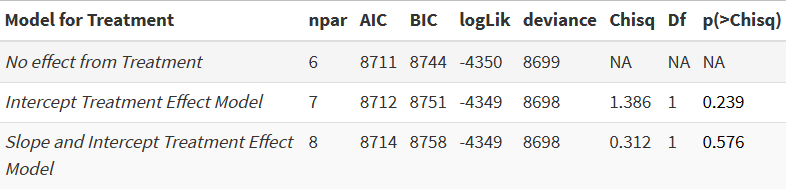
\includegraphics[width = \textwidth]{model_anova.png}
\centering
\caption{Output of Likelihood Ratio test generated by R sequentially comparing the above models}
\end{figure}

At our $\alpha = 0.05$, we failed to reject the null hypothesis for either of our new models, meaning we did not have sufficient evidence to say that differences in the treatment group lead to different intercepts or slopes in our model for toenail growth over time. We can therefore conclude that there is no significant evidence that one treatment is superior to the other.

Although, there is no significant difference in the progression of toenail growth based on treatment, we can still use our null model to predict the progression of toenail growth in response to either of the two treatments. The output of our model is given in \textbf{Fig. 2}.

\begin{figure}[H]
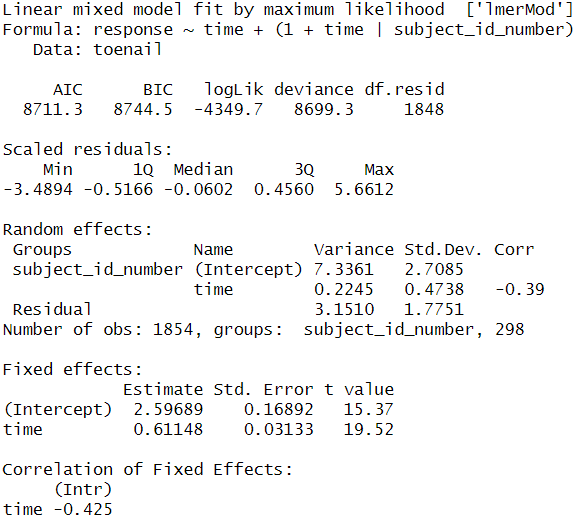
\includegraphics[scale=0.7]{model.png}
\centering
\caption{Output of our no progression model in LME4}
\end{figure}

We can see from this that there is a correlation coefficient of $-0.39$ between the random effect on slope and the random effect on intercept from subject ID. We can also see that our model's estimate for $\gamma_{00}$ is $2.59689$, the estimate for $\gamma_{10}$ is $0.61148$. This will allow us to make predictions about the progression of toenail growth in a number of situations. The first is for extrapolating a particular known subject in the study's continued progression over time. In which case we can use the null model's predicted coefficients for the fixed time effect, and the model's estimates for each subjects random variables. We can see this applied in \textbf{Eq. 4}. 

The second is for predicting a new subject's toenail size at a given time given no previous data. For this we avoid using any prediction for the random coefficients, since we have no prior information and instead use only the predicted estimated for the fixed time effect. The equation for this can be found in \textbf{Eq. 5} The advantage of using this mixed effect model instead of a simple linear regression is that the mixed effect model will shrink the subject related effects towards zero. This means that our mixed effect model will not be as effected by an extreme subject differences. This can be visualized in \textbf{Fig. 2}

\begin{equation}
    \hat{y}_{i} = 2.5969 + b_{0i} + (0.6115 + b_{1i})(\textrm{Time}) 
\end{equation}
\begin{center}
    \textit{Where both $b_{0i}$ and $b_{1i}$ are predicted by our LME4 model for each subject.}
\end{center}

\hspace{10mm} 

\begin{equation}
    \hat{y}_{i} = 2.5969 + 0.6115(\textrm{Time})
\end{equation}

\begin{figure}[H]
\includesvg[width = \textwidth]{combine.svg}
\centering
\caption{\textbf{Left}: Comparison of each subject's predicted slope and intercept based on a simple linear regression (\textit{orange}) and based on the full mixed effects model (\textit{blue}). \textbf{Right}: Visualization of the connection between $b_{0i}$ and $b_{1i}$ predicted by our mixed effects models for all of the subjects (\textit{blue})}
\end{figure}

\hspace{10mm} The final situation is for predicting a new subject's evolution over time given the starting size at month 0. Our model gives that the correlation coefficient between the two random variables $b_{0i}$ and $b_{1i}$ is $-0.39$, this means with information about the starting intercept of a new subject we can create a prediction for the random effect on slope. The connection between these coefficients is visualized in \textbf{Fig. 2}. We created a new linear regression between $b_{0i}$ and $b_{1i}$, which yielded the following equation:
\begin{equation*}
    \hat{b}_{1i} = -0.058\hat{b}_{0i}
\end{equation*}
Since we can estimate the random effect on the intercept from the given intercept, $I_i$ via the following
\begin{align*}
    & I_{i} = \gamma_{00} + \hat{b}_{0i} \implies\\
    & \hat{b}_{1i} = I_{i} - \gamma_{00}
\end{align*}
We can create a new model as follows, with $\gamma$ as our predicted intercept coefficient from the model
\begin{equation}
    \hat{y}_i = I_i +(0.6115 + 0.058[I_i - 2.5969])(\textrm{Time})
\end{equation}

\end{document}